\begin{figure}
\centering
\begin{tikzpicture}[scale=0.75,transform shape]
\GraphInit[vstyle=Simple]
\SetGraphUnit{2.5}
\Vertex[a=45,d=2.5]{A}
\Vertex[a=135,d=2.5]{B}
\Vertex[a=225,d=2.5]{C}
\Vertex[a=315,d=2.5]{D}
\Edge[label=$e_1$](A)(B)
\Edge[label=$e_2$](B)(C)
\Edge[label=$e_4$](B)(D)
\Edge[label=$e_3$](C)(D)
\end{tikzpicture}

\caption{Consider the cycle matroid $M(G)$ of the graph above. The collection
of independent sets of $M(G)$ are exactly the subsets of the edge set of $G$
which do not contain any cycles. Thus $\I = \{$$e_1,e_2,e_3,e_4,e_5,$$\{e_1,e_2\},$
$\{e_1,e_3\},$$\{e_1,e_4\},$$\{e_2,e_3\},$$\{e_2,e_4\},$$\{e_3,e_4\},$$\{e_1,e_2,e_3\},$$
\{e_1,e_2,e_4\},$$\{e_1,e_3,e_4\}$$\}$, where $\I$ is the independent set of
$M(G)$. Note that $\{e_2,e_3,e_4\} \not\in \I$ as the edges $e_2$, $e_3$ and
$e_4$ form a cycle in $G$.}
\label{fig:cycle-matroid-example}
\end{figure}
